\documentclass{article}
\usepackage{amsmath}
\usepackage{setspace}
\usepackage{hyperref}
\usepackage{mathrsfs}
\usepackage{graphicx}
\usepackage[utf8]{inputenc}

% Default fixed font does not support bold face
\DeclareFixedFont{\ttb}{T1}{txtt}{bx}{n}{12} % for bold
\DeclareFixedFont{\ttm}{T1}{txtt}{m}{n}{12}  % for normal

% Custom colors
\usepackage{color}
\definecolor{deepblue}{rgb}{0,0,0.5}
\definecolor{deepred}{rgb}{0.6,0,0}
\definecolor{deepgreen}{rgb}{0,0.5,0}

\usepackage{listings}

% Python style for highlighting
\newcommand\pythonstyle{\lstset{
		language=Python,
		basicstyle=\ttm,
		otherkeywords={self},             % Add keywords here
		keywordstyle=\ttb\color{deepblue},
		emph={MyClass,__init__},          % Custom highlighting
		emphstyle=\ttb\color{deepred},    % Custom highlighting style
		stringstyle=\color{deepgreen},
		frame=tb,                         % Any extra options here
		showstringspaces=false            % 
}}


% Python environment
\lstnewenvironment{python}[1][]
{
	\pythonstyle
	\lstset{#1}
}
{}

% Python for external files
\newcommand\pythonexternal[2][]{{
		\pythonstyle
		\lstinputlisting[#1]{#2}}}

% Python for inline
\newcommand\pythoninline[1]{{\pythonstyle\lstinline!#1!}}
\graphicspath{{./figures/}}

%\usepackage[letter,margin=1.5in]{geometry}
%\addtolength{\rightmargin}{-0.5in}
%\addtolength{\textwidth}{0.5in}
%\addtolength{\oddsidemargin}{-.875in}
%\addtolength{\evensidemargin}{-.875in}
%\addtolength{\textheight}{1.75in}

\makeatletter
\renewcommand\section{\clearpage\newpage\@startsection {section}{1}{\z@}%
	{-3.5ex \@plus -1ex \@minus -.2ex}%
	{2.3ex \@plus.2ex}%
	{\normalfont\Large\bfseries}}
\makeatother

\begin{document}

%==========================================================================
%==========================================================================
% Title pages.

\newcommand{\mytitle}{[title]}
\newcommand{\myauthor}{Reece Humphreys}
\newcommand{\myadvisor}{Dr. Yaouen Fily}

\newcommand{\myskip}{\vspace{0.5in}}
\newcommand{\layouttitle}[1]{{\bf\large\MakeUppercase{#1}}}
\setlength{\parindent}{0em}
\doublespace
\pagenumbering{roman}
\thispagestyle{empty}

\begin{center}

	\vspace{4in} 
	\layouttitle{\mytitle} \\ by \\ \myauthor
	
	\vspace{1in}
	A Thesis Submitted to the Faculty of \\
	The Wilkes Honors College \\
	in Partial Fulfillment of the Requirements for the Degree of \\
	Bachelor of Science in Liberal Arts and Sciences \\
	with a Concentration in Physics \\ 
	\vspace{1in} 
	Wilkes Honors College of \\
	Florida Atlantic University \\
	Jupiter, Florida \\
	May \number\year

\end{center}

\newpage

%==========================================================================

\vspace{4in}
\begin{center}
	\layouttitle{\mytitle} \\
	by \\
	\myauthor
\end{center}

\singlespace
\vspace{1in}
This thesis was prepared under the direction of the candidate's thesis advisor, \myadvisor, and has been approved by the members of their supervisory committee. It was submitted to the faculty of the Harriet L. Wilkes Honors College and was accepted in partial fulfillment of the requirements for the degree of Bachelor of Science in Liberal Arts and Sciences.

\vspace{1in}
SUPERVISORY COMMITTEE:

\newcommand{\myrule}{\vspace{0.5in}\rule{4in}{0.5pt} \\}

\myrule
\myadvisor

\myrule 
{}[second reader]

\myrule
Interim Dean Timothy Steigenga, Harriet L. Wilkes Honors College 

\myrule
Date

\newpage

%==========================================================================

%\begin{center}
%	\layouttitle{Acknowledgements}
%\end{center}
\section*{Acknowledgments}
%\addcontentsline{toc}{section}{Acknowledgements}

\myskip
Some acknowledgments.

\newpage

%==========================================================================

%\begin{center}
%	\layouttitle{Abstract}
%\end{center}
\section*{Abstract}
\addcontentsline{toc}{section}{Abstract}

\myskip
\renewcommand{\arraystretch}{1.5}
\begin{tabular}{@{}l@{\hspace{3ex}}l}
	Author: & \myauthor \\
	Title: & \mytitle \\
	Institution: & Harriet L. Wilkes Honors College, Florida Atlantic University \\
	Thesis Advisor: & \myadvisor \\
	Degree: & Bachelor of Science in Liberal Arts and Sciences \\
	Concentration: & Mathematics \\
	Year: & \the\year
\end{tabular}


\myskip
\doublespace
Orbital debris has quickly become one of the newest sources of pollution as a result of mankind's desire to work in, explore, and utilize space. However, unlike most types of pollution which people experience daily, this is pollution that is impossible for the average person to ever encounter, yet poses just as grand of a threat as the other types. Orbital debris are the remnants of orbital collisions, weapons tests, decommissioned satellites, and spent rocket stages that are passing over our heads faster than bullets and containing similar energy to hand grenades. This paper explores the existing models of orbital debris generation, how clouds of debris evolve with respect to time, and the ramifications that they pose.
\singlespace
\newpage

%==========================================================================

\tableofcontents

\listoftables

\listoffigures


%==========================================================================

\setlength{\parindent}{1em}
\pagenumbering{arabic}

%==========================================================================
%==========================================================================
% Thesis proper.


\section{Introduction}
\label{introduction}
\doublespace
\subsection{Motivation}
Due to the accelerating launch cadence in the space sector, increased accessibility and resources for small teams to create cube satellites, and satellite mega constellation constructions underway, researchers have become increasingly concerned about the implications of potential orbital collisions. These worries have been compounded by the actions taken by foreign nations with regards to anti-satellite weapons which create substantial amounts of debris. In one such instance, a 2007 Chinese anti-satellite missile test was universally condemned and received statements from government officials such as U.K. prime minister who stated "We are concerned about the impact of debris in space and we expressed that concern”. These fragmentation events can be difficult to track due to the small size of some of the debris fragments that are generated, yet they can pose a great hazard to other satellites and crewed operations being conducted in space. Tens of millions of pieces of orbital debris currently exist within Low Earth Orbit (LEO) with an average size smaller than 1cm. While minuscule in size, these pieces of debris have an average impact velocity of 10 km/s which generates similar energy to that of an exploding hand grenade. It is, therefore, paramount to study the phenomena that arise within orbital debris clouds to gather methods for mitigating debris cloud formations. Without such a study, the future commercialization of space, the potential for humanity to become a multi-planetary species, and the benefits that the advanced satellites provide researchers will remain in jeopardy.
\subsection{Methodology}
To model how debris clouds propagate over time, a method of simulating the debris generated by a collision or explosion is required. Breakup models use observations of orbital collisions to create statistical models that predict the size, mass, speed, and number of debris pieces generated.  Once these characteristics of each debris piece are obtained, equations of motion can be implemented that account for the significant forces acting on each debris fragment, such as drag and solar radiation, to model how the debris position and velocity will evolve over time. This paper implements the NASA Standard Satellite Breakup Model (Source) to simulate the orbital collisions and gather information regarding the behavior of orbital debris. This was accomplished by utilizing the model to create an implementation in python which has been made \href{https://github.com/ReeceHumphreys/OrbitalDebris}{open source on GitHub} for others wishing to build on the foundations of this research.

Following the implementation of the breakup model, the implementation of dominant orbital perturbations is given. These are forces that act on debris to change their orbits over time and include effects such as atmospheric drag and solar radiation. The optimal way to represent these effects is through changes in orbital parameters, which is an alternate way of expressing the current state of an object rather than using euclidean coordinates $(x,y,z, v_x, v_y, v_z)$ . The benefits of using orbital parameters is explored more in-depth later in the paper.

Finally a case study showing the magnitude of orbital collisions is shown along with an analysis on the potential for the Kessler syndrome to occur given the increase in launch cadence and recent expansions into constructing satellite mega constellations.

  
\subsection{Past research and Roadmap}
*** Include what past researchers have explored and where my research fits in*** \newline
An outline of the roadmap for this paper is as follows: \newline 
\textbf{Chapter 1:}  \newline 
\textbf{Chapter 2:}  \newline 
\textbf{Chapter 3:}  \newline 
\textbf{Chapter 4:}   \newline 
\singlespace

\section{Modeling Satellite Breakups}
\label{Modeling Satellite Breakups}
\doublespace


\subsection{The NASA Standard Satellite Breakup Model}

A satellite is any artificial body placed in orbit around the earth or moon or another planet. The definition of the term is intentionally general and as such, can be used to reference space craft (SC), remnants of rockets (RB), and communication devices (SAT) in orbit.  A satellite breakup model is a mathematical model used to describe the outcome of a a satellite breakup due to an explosion or a collision (Liou, 2012) \cite{jer_chyi_liou_orbital_nodate}.  The outcome of any satellite breakup model should be a set of characteristics that should describe the size, area-to-mass (AM) ratio, and the ejection velocity of each fragment produced in the satellite breakup (Johnson and Krisko, 2001) \cite{johnson_nasas_2001}. The NASA Standard Satellite Breakup Model is an industry standard breakup model developed by NASA and is used by most major space agencies such as the European Space Agency (ESA) and the Japanese Aerospace Exploration Agency (JAXA). The implementation of it was provided by Johnson et. al in 2001 \cite{johnson_nasas_2001} but was later clarified by Kristo in 2011 \cite{krisko_proper_2011}. 

The way that the model works is by using experimental observations performed both on Earth and in orbit to characterize the breakup using statistical distributions. The reason being is breakup events are stochastic, i.e are nondeterministic.  For example, explosions are stochastic, they do not occur the same way every time.  By using a statistical distribution and sampling from it we can more accurately represent the fragments that would be generated during a collision or explosion. For this paper, I will be focusing on how the collision fragments are generated, but it should be noted that the explosion case just involves slightly different parameters in many cases.

%==========================================================================

%\section{Single Photon Down Conversion}
%
%
%\begin{gather}
%	|\psi_R\rangle = r|\psi_A\rangle +t|\psi_B\rangle 
%	\label{eq:first} \\
%	|\psi_T\rangle = t|\psi_A\rangle +r|\psi_B\rangle 
%	\label{eq:second} \\
%	P_A=\langle\psi_A|\psi_{input}\rangle^2
%	\label{eq:third}
%\end{gather}
%
%Equations \eqref{eq:first}-\eqref{eq:second} describe some kind of decomposition of a quantum state on a basis. 
%Equation \eqref{eq:third} is some kind of probability.
%As discussed in section \ref{introduction}...

%\section{A table and a figure}

%\subsection{A table}

%\begin{table}[h]
%	\centering
%	\begin{tabular}{|c|c|c|} \hline
%		I guess & I have & to make \\ \hline
%		a table & now & ... \\ \hline
%	\end{tabular}
%	\caption{Test table.}
%\end{table}

%\subsection{A figure}

%\begin{figure}[h]
%	\centering
%	
\includegraphics[width=0.4\linewidth]{honors_college}
%	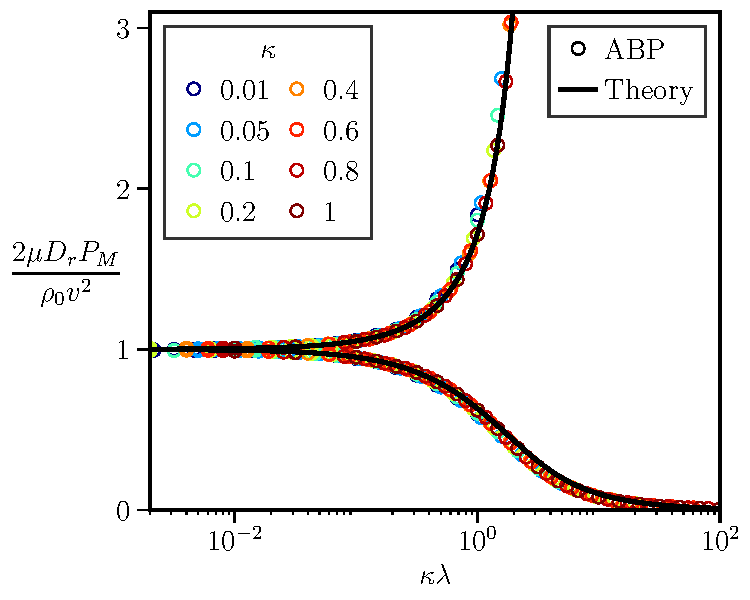
\includegraphics[width=0.4\linewidth]{fig1_2a_pour_yariv}
%	\caption{Test figure.}
%\end{figure}
%

%It all becomes clear if you read \cite{Fily2017}.


%==========================================================================
%==========================================================================
% Appendices

\appendix

\section{An appendix}

%==========================================================================

\section{An other appendix}

%==========================================================================
%==========================================================================
% Bibliography.

% Some other possible styles: abbrv, acm, alpha, apalike, ieeetr, plain, siam, unsrt
\bibliographystyle{plain}
\bibliography{honors_thesis_bibliography} % Use the name of you bibliography file. Omit the ".bib" extension.

\end{document}

